\section{\texorpdfstring{\Gls{spade}}{SPADe} flow overview}
\label{chap:spadeoverview}
This thesis presents a scenario- and platform-aware design flow (\gls{spade}) for \gls{ibc} systems that brings together the essence of key scientific contributions made in this thesis (explained in Section~\ref{chap:challenges}).
An overview of our \gls{spade} approach is illustrated in Fig.~\ref{fig:ch1_spade_overview}, summarised below and explained in detail in subsequent chapters.

\begin{figure}[ht]
\centerline{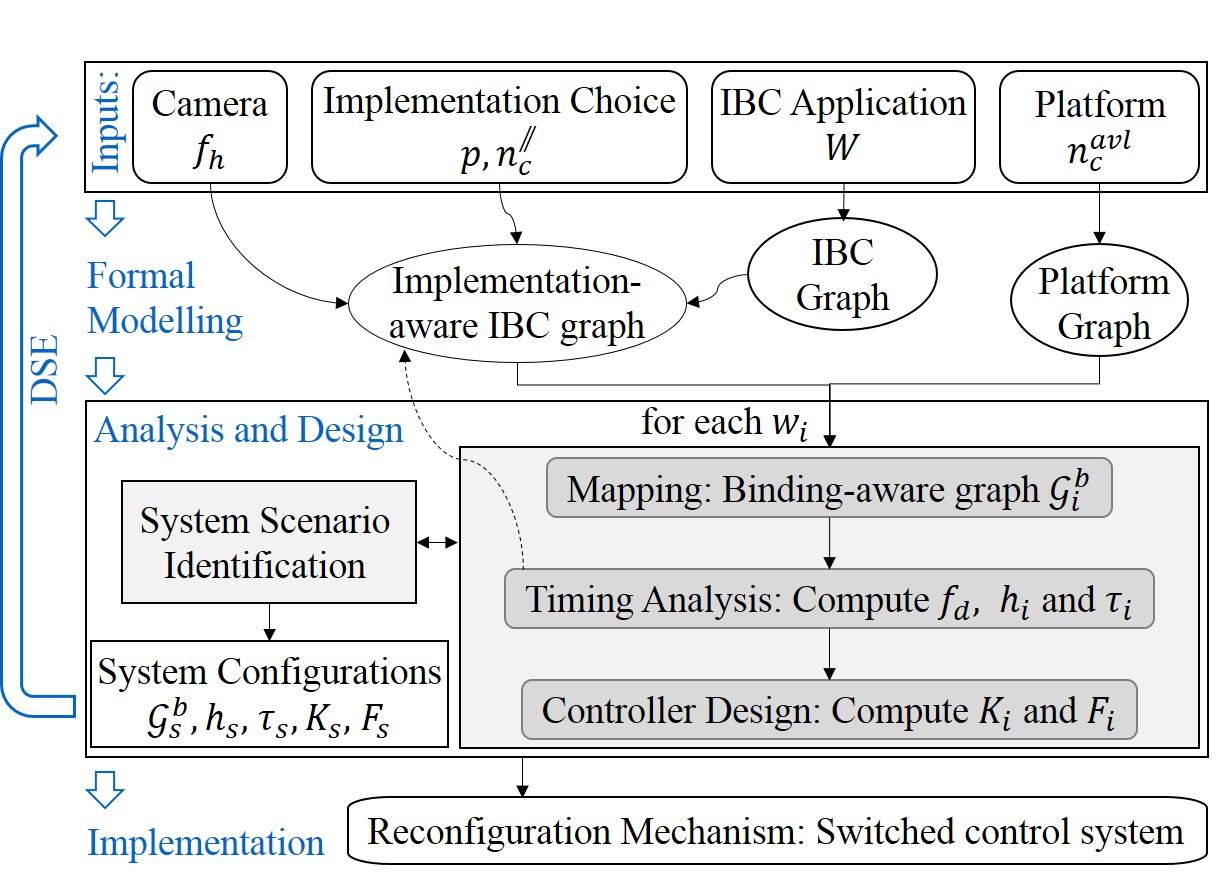
\includegraphics[width=\textwidth]{01_intro/images/SPADeOverview5.jpg}}
%\vspace{-1ex}
\caption{Overview of our \gls{spade} design flow for pipelined parallelism. $\setW$ is the set of varying workloads and $\aWorkload_i,\ \bindingAwareSDFG{i},\ \tau_i,\ h_i, \Kgain_i$ and $\Fgain_i$ are the workload, binding-aware graph, sensor-to-actuator delay, sampling period, feedback gain and feedforward gain for a workload scenario $s_i$ (determined by $\aWorkload_i\in \setW$); 
$\bindingAwareSDFG{s},\ \tau_s,\ h_s, \Kgain_s$ and $\Fgain_s$ are the corresponding parameters for an identified system scenario $s_s$ (that abstract multiple workload scenarios). $\fh$ is the camera frame arrival period, $\fd$ is the inter-frame dependence time, $p$ is the number of pipes for pipelining, $\numCoresParallel$ is the number of cores allocated for parallelism per pipe, and $\numCoresAvailable$ is the total number of available cores. For the scope of the thesis, the pipelined implementation is always periodic.}
\label{fig:ch1_spade_overview}
%\vspace{-1em}
\end{figure}
\begin{enumerate}
    \item Formal modelling of the \gls{ibc} system: An \gls{ibc} application is captured as an \gls{ibc} \gls{sadf} considering workload variations $\setW$ and the platform as a platform graph. Further, an \emph{implementation-aware} \gls{ibc} \gls{sadf} captures the given design parameters - camera frame arrival period $\fh$, maximum number of allowed pipes $\numPipes$, total number of available cores $\numCoresAvailable$ and allocated processing cores for parallel execution per pipe $\numCoresParallel$.
    The design parameters fully determine the implementation choice - non-pipelined without parallelism, non-pipelined with parallelism, pipelined without par\-al\-lelism and pipelined with parallelism. The parallelism here refers to the parallel execution of sensing subtasks limited by the degree of parallelism of the \gls{ibc} application.
    \item Analysis and design: We map the implementation-aware \gls{ibc} graph for each workload $\workloadScenario \in \setW$ to the platform graph to obtain the \emph{binding-aware graph} $\bindingAwareSDFG{i}$ for that specific workload using the SDF3 mapping flow~\cite{stuijk2007}. 
    $\bindingAwareSDFG{i}$ is a \gls{sdfg} that models the mapping of the implemen\-tation-aware graph to the platform graph. The mapping binds each actor in the \gls{sdfg} to a processing core in the platform graph. For the ordering of execution of actors bound to the same core, a static-order schedule is encoded in the \gls{sdfg}.
    A throughput and latency analysis of $\bindingAwareSDFG{i}$ yields the sensor-to-actuator delay $\tau_i$, and sampling period $h_i$.
    For a pipelined implementation, the throughput analysis of the worst-case image-workload scenario allows to compute the inter-frame dependence time $\fd$ (explained later in Section~\ref{sec:ch7_IFD}). 
    If $\fd>h_i$, the implementation-aware graph is updated with the realisable period and $\tau_i$ and $h_i$ are recomputed. 
     The controllers are then designed for the resulting $(\tau_i,\ h_i)$ to obtain the controller feedback and feedforward gains $(\Kgain_i,\ \Fgain_i)$.
     Trying to cater to the designed workload scenarios at runtime means that we have a switching system. A switching system with too many switching states is challenging for controller stability and may result in poor performance. 
     Hence, we aggregate multiple workload scenarios with similar control timing parameters as a \emph{system scenario}.
    A system scenario $\sysScenario$ abstracts multiple workload scenarios and has a constant $(\tau_s,\ h_s)$ during implementation. A \emph{system configuration} is defined as the combination of mapping and controller configurations, i.e. $\bindingAwareSDFG{s}$, $\tau_s,\ h_s,\ \Kgain_s,$ and $\Fgain_s$ (as explained later in Section~\ref{sec:ch7_sysConfigStability}).
    It should be noted that the controller gains (i.e.,  $\Kgain_s$, and $\Fgain_s$) can be designed using different approaches depending on the design goals.
    In this thesis, the \gls{spade} flow is illustrated using the \gls{lqr}, \gls{lqi}, \gls{lqg}, \gls{mpc}, and \gls{mjls} controller design approaches.
    Typically, the number of identified system scenarios is low in number, and the idea is that switching between the system scenarios at runtime guarantees stability and improved performance.
    For pipelined parallelism, a \gls{dse} using the \gls{spade} flow needs to be performed by varying the design parameters to identify the best implementation choice (parameters $\numPipes, \numCoresParallel$, further explained in Section~\ref{sec:ch7_DSE}).
    \item Runtime implementation: The system configurations for the implementation choice are stored in a \gls{lut} in platform memory for the runtime implementation. Dynamic runtime reconfiguration may be needed since there can be a switching behaviour between system configurations due to image-workload variations.
\end{enumerate}